\chapter{Manual Annotation} \label{chapter:manual_annotation}

\begin{figure}[!tbp]
	\centering
    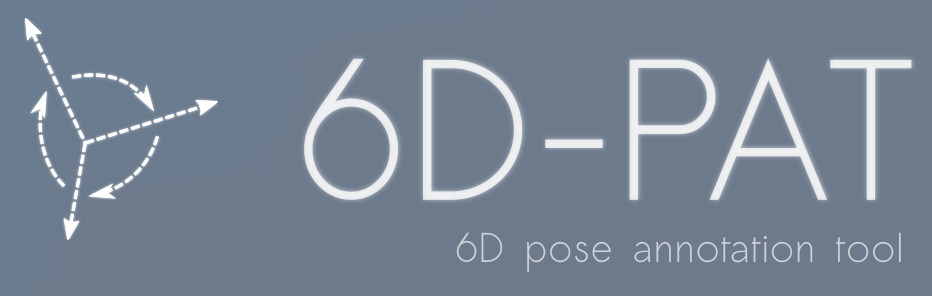
\includegraphics[width=\linewidth]{6dpat}
    \caption{The logo of the pose annotation tool 6D-PAT. Own image.}
    	\label{fig:6dpat_logo}
\end{figure} 

The following chapter analyzes the manual 6D pose annotation process and its prerequisites. To this end, we define the necessary terminology and explain the workflow of recovering poses from images using the developed tool. 

\section{Terminology} \label{section:terminology}

\textbf{Image.} An image $I$ is a 2D matrix of pixels. The pixel $u$ at position $(i, j)$ is referenced by the tuple $(x, y)$, where $x = j$ and $y = i$. The inverted notation is chosen over the row-major matrix indexing because images are often column-major indexed. \\

\noindent\textbf{Object Model.} An \textit{object model} (or \textit{3D model}) $O$ is composed of a set of points $M \subseteq \mathbb{R}^3$ and a set of triangles $T \subseteq M^3$, also called a mesh. The type of object is not restricted. In the T-Less dataset \cite{tless} the objects are mostly screws and other hardware. \\

\noindent\textbf{6D Pose.} A \textit{6D pose} $P$ is the tuple $(R, t)$, where $R$ is the 3x3 rotation matrix and $t$ the translation vector used to transform an object model into camera coordinates (see Section \ref{objectcoordinates}). \\

\noindent\textbf{Correspondence.} A \textit{correspondence} $C$ is the tuple $(u, p)$, which captures the relation between a pixel $u$ of an image $I$ and an object model $O$. The pixel $u$ is the projection of the 3D point $p$ on the surface of $O$ onto the image plane using the camera matrix $K$ and a pose $P$. A pose can be retrieved computationally if at least three correspondences are known (see Section \ref{objectcoordinates}). \\

\noindent\textbf{Segmentation Mask.} A \textit{segmentation mask} (or \textit{segmentation image}) $S$ for an image $I$ is a second image of the same size. Each position $(x, y)$ of the mask encodes the class of the pixel at $(x, y)$ in $I$. The set of classes can be defined arbitrarily. In the context of this work each class represents a type of object model. The segmentation mask can be seen as the mapping $s(x, y) = q_i$ for a class set $Q = \{q_0, \cdots, q_n\}$. \\

\noindent\textbf{Ground-Truth.} A \textit{ground-truth pose} $\bar{P}$ is a 6D pose. A ground-truth pose is always recovered by a human instead of a machine. The ground-truth pose is the best approximation of the rotation and translation of an object model $O$ visible in an image $I$. It is an approximation because there can be a discrepancy between the real world object and its digital 3D representation and because image conditions like lightning, motion blur, etc. might make it unfeasible to recover the perfect pose. Distortions by the camera used to photograph the object and other influences might also not be modeled correctly or not accounted for at all. But it must apply that the translation and rotation error of a ground-truth pose $\bar{P}$ are within a certain threshold. \\

\noindent\textbf{Depth Image.} A \textit{depth image} is an image $D$ belonging to an image $I$ of the same size that contains the distance $d$ of the camera to the surface for each pixel $u$ in $I$. Depth images can be obtained using special cameras or from stereo images and are often used in pose estimation and other computer vision tasks. A depth image can also be denoted by "RGB-D".

\begin{figure}[!tbp]
	\centering
	\begin{subfigure}[t]{0.47\textwidth}
	\centering
    	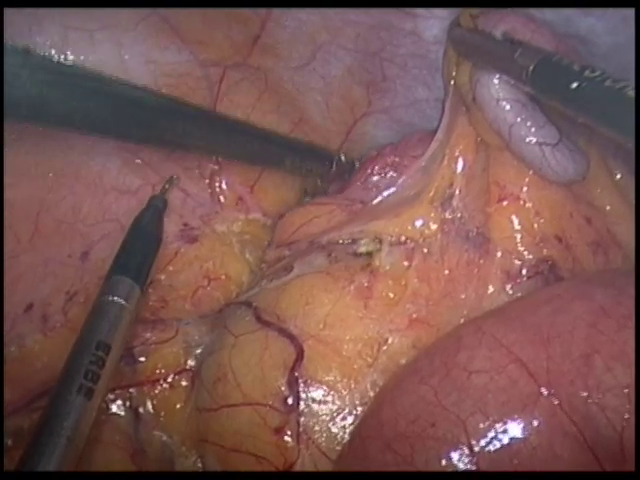
\includegraphics[width=0.8\linewidth]{sfb_original}
    	\caption{An example image from the Endoscopic Vision Challenge dataset. Image from \cite{endovis}.}
    	\label{fig:sfb_original}
	\end{subfigure}
	\hfill
	\begin{subfigure}[t]{0.47\textwidth}
	\centering
    	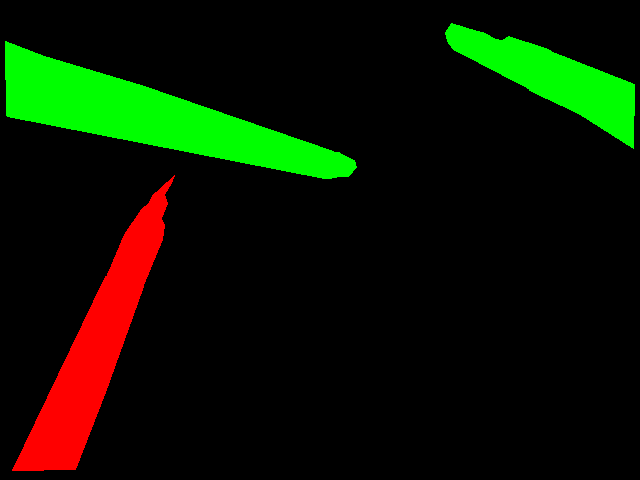
\includegraphics[width=0.8\linewidth]{sfb_segmentation}
    	\caption{The corresponding segmentation mask to the image in fig \ref{fig:sfb_original}. The colors encode the tools' classes. Image from \cite{endovis}.}
    	\label{fig:sfb_segmentation}
	\end{subfigure}
	\caption{An example image and its corresponding segmentation mask from the Endoscopic Vision Challenge dataset.}
	\label{fig:sfb}
\end{figure} 

\section{Images of the Endoscopic Vision Challenge}

The goal of this work is to provide a system to successfully and efficiently annotate the images of the Endoscopic Vision Challenge. The dataset includes segmentation masks but no object models or existing pose annotations. An example image together with the corresponding segmentation mask are given in \fig \ref{fig:sfb}. The dataset does not provide depth images and occlusion and artifacts like motion blur can occur in the images. The issues with this dataset and why it was not fully annotated is discussed in Section \ref{section:6dpat_difficulties}. 

\section{6D Pose Annotation Tool (6D-PAT)}

The creation of sufficient training data for neural networks can be a time-consuming and tedious process. Using non-specialized tools designed for other purposes, like 3D modeling or CAD programs, require the person creating the annotations to get accustomed to complex user interfaces (\gls{ui}s). The goal of the annotation tool is to provide a system that allows easy and efficient annotation of images - images of the Endoscopic Vision Challenge in particular. The ground-truth poses recovered using the program can then be used to train a neural network. The program is written mainly in the language C++ and named \textit{6D - Pose Annotation Tool (\gls{6dpat})}. Its logo can be seen in \fig \ref{fig:6dpat_logo}. We developed the program on the \textit{Linux}-based operating system \textit{Ubuntu} but it is compatible to other operating systems, as well.

\subsection{Frameworks \& Third-Party Libraries}

The listed frameworks are all the necessary dependencies of the annotation tool. There are no other dependencies. The user needs to compile or install the dependencies before using the annotation tool. But since all frameworks/libraries are platform-independent the program can be compiled and run on different systems. \\

\noindent\textbf{Qt.} \textit{Qt} \cite{qt} is a powerful framework for C++ that offers a vast selection of user interface components but also general functionality that exceeds the capabilities of the standard C++ library. Qt was also chosen as the main framework because it ensures portability of C++ applications by encapsulating system calls of all kind. The program \textit{Qt Creator} is the \textit{Integrated Development Environment (IDE)} that is included in the Qt distribution. Qt Creator was used to write and execute the code of \gls{6dpat}. \\

\begin{figure}[!tbp]
	\centering
	\begin{subfigure}[t]{0.47\textwidth}
		\centering
    	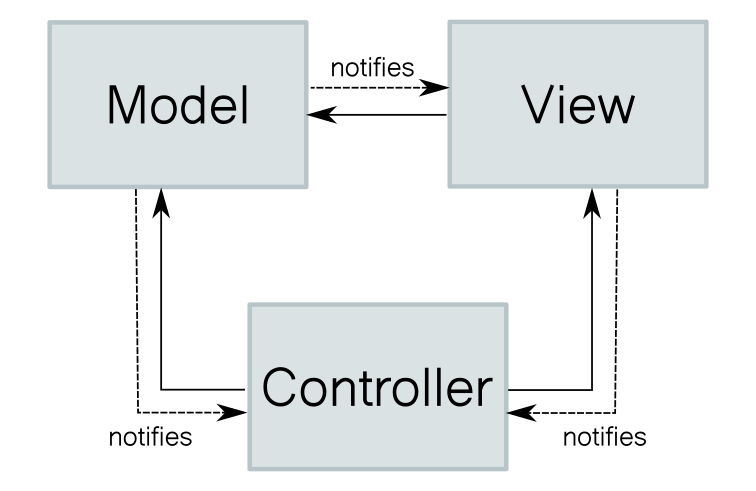
\includegraphics[width=0.8\linewidth]{mvc}
    	\caption{The Model-View-Controller architecture. The solid lines stand for a direct connection either because the target is owned or known by reference. The dashed line is an indirect connection using for example the observer pattern or the Qt Signals and Slots mechanism visible in \fig \ref{fig:qt_signals_slots}. Own image.}
    	\label{fig:mvc}
	\end{subfigure}
	\hfill
	\begin{subfigure}[t]{0.47\textwidth}
	\centering
    	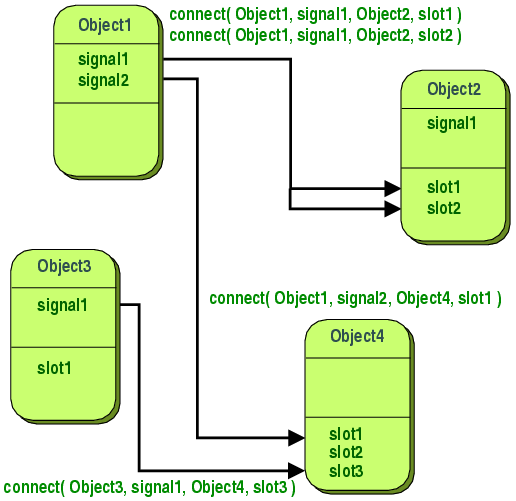
\includegraphics[width=0.8\linewidth]{qt_signals_slots}
    	\caption{The Signals and Slots mechanism of Qt. A class can define signals which can be emitted. Slots are functions that can be connected to signals. When a signal is emitted, all connected slots will be called. Image from \cite{qt_signals_and_slots}.}
    	\label{fig:qt_signals_slots}
	\end{subfigure}
	\caption{Two basic architectural concepts used in \gls{6dpat}: the model view controller pattern and the signal and slots pattern.}
\end{figure} 

\noindent\textbf{OpenGL.} \textit{OpenGL} \cite{opengl} is a widespread open-source 3D graphics library specification. Implementations of the specification exist for many different operating systems, which makes OpenGL-using applications portable. \\

\noindent\textbf{OpenCV.} \textit{OpenCV} \cite{opencv} is a C++ library created for various computer vision tasks, hence the name. OpenCV provides functions for tracking, object detection, segmentation and many more. We use its \textit{solvePnPRansac} method in this work. \\ 

\noindent\textbf{Assimp.} \textit{Assimp} \cite{assimp} is a C++ library designed to import 3D models. The library was incorporated into the tool to ensure a broad support of 3D model formats.

\subsection{Architecture \& Code Design}

\gls{6dpat} is primarily a \textit{Graphical User Interface (GUI)} program, i.e. its purpose is to display a window and enable optical interaction of the user, like clicking. Thus, we chose the \textit{Model-View-Controller (\gls{mvc})} pattern as the underlying architecture. \gls{mvc} separates the concerns of data management (Model), displaying data (View) and high level logic (Controller). The schematic of the \gls{mvc} architecture is given in \fig \ref{fig:mvc}. The indirect connections are realized via Qt's signals and slots mechanism, which is visualized in \fig \ref{fig:qt_signals_slots}. To speed up interface creation, we used \textit{Qt Designer} to layout the views. Qt Designer is a graphical tool that allows placement of UI components and linking of signals and slots without directly writing code.

\begin{figure}[!tbp]
	\centering
    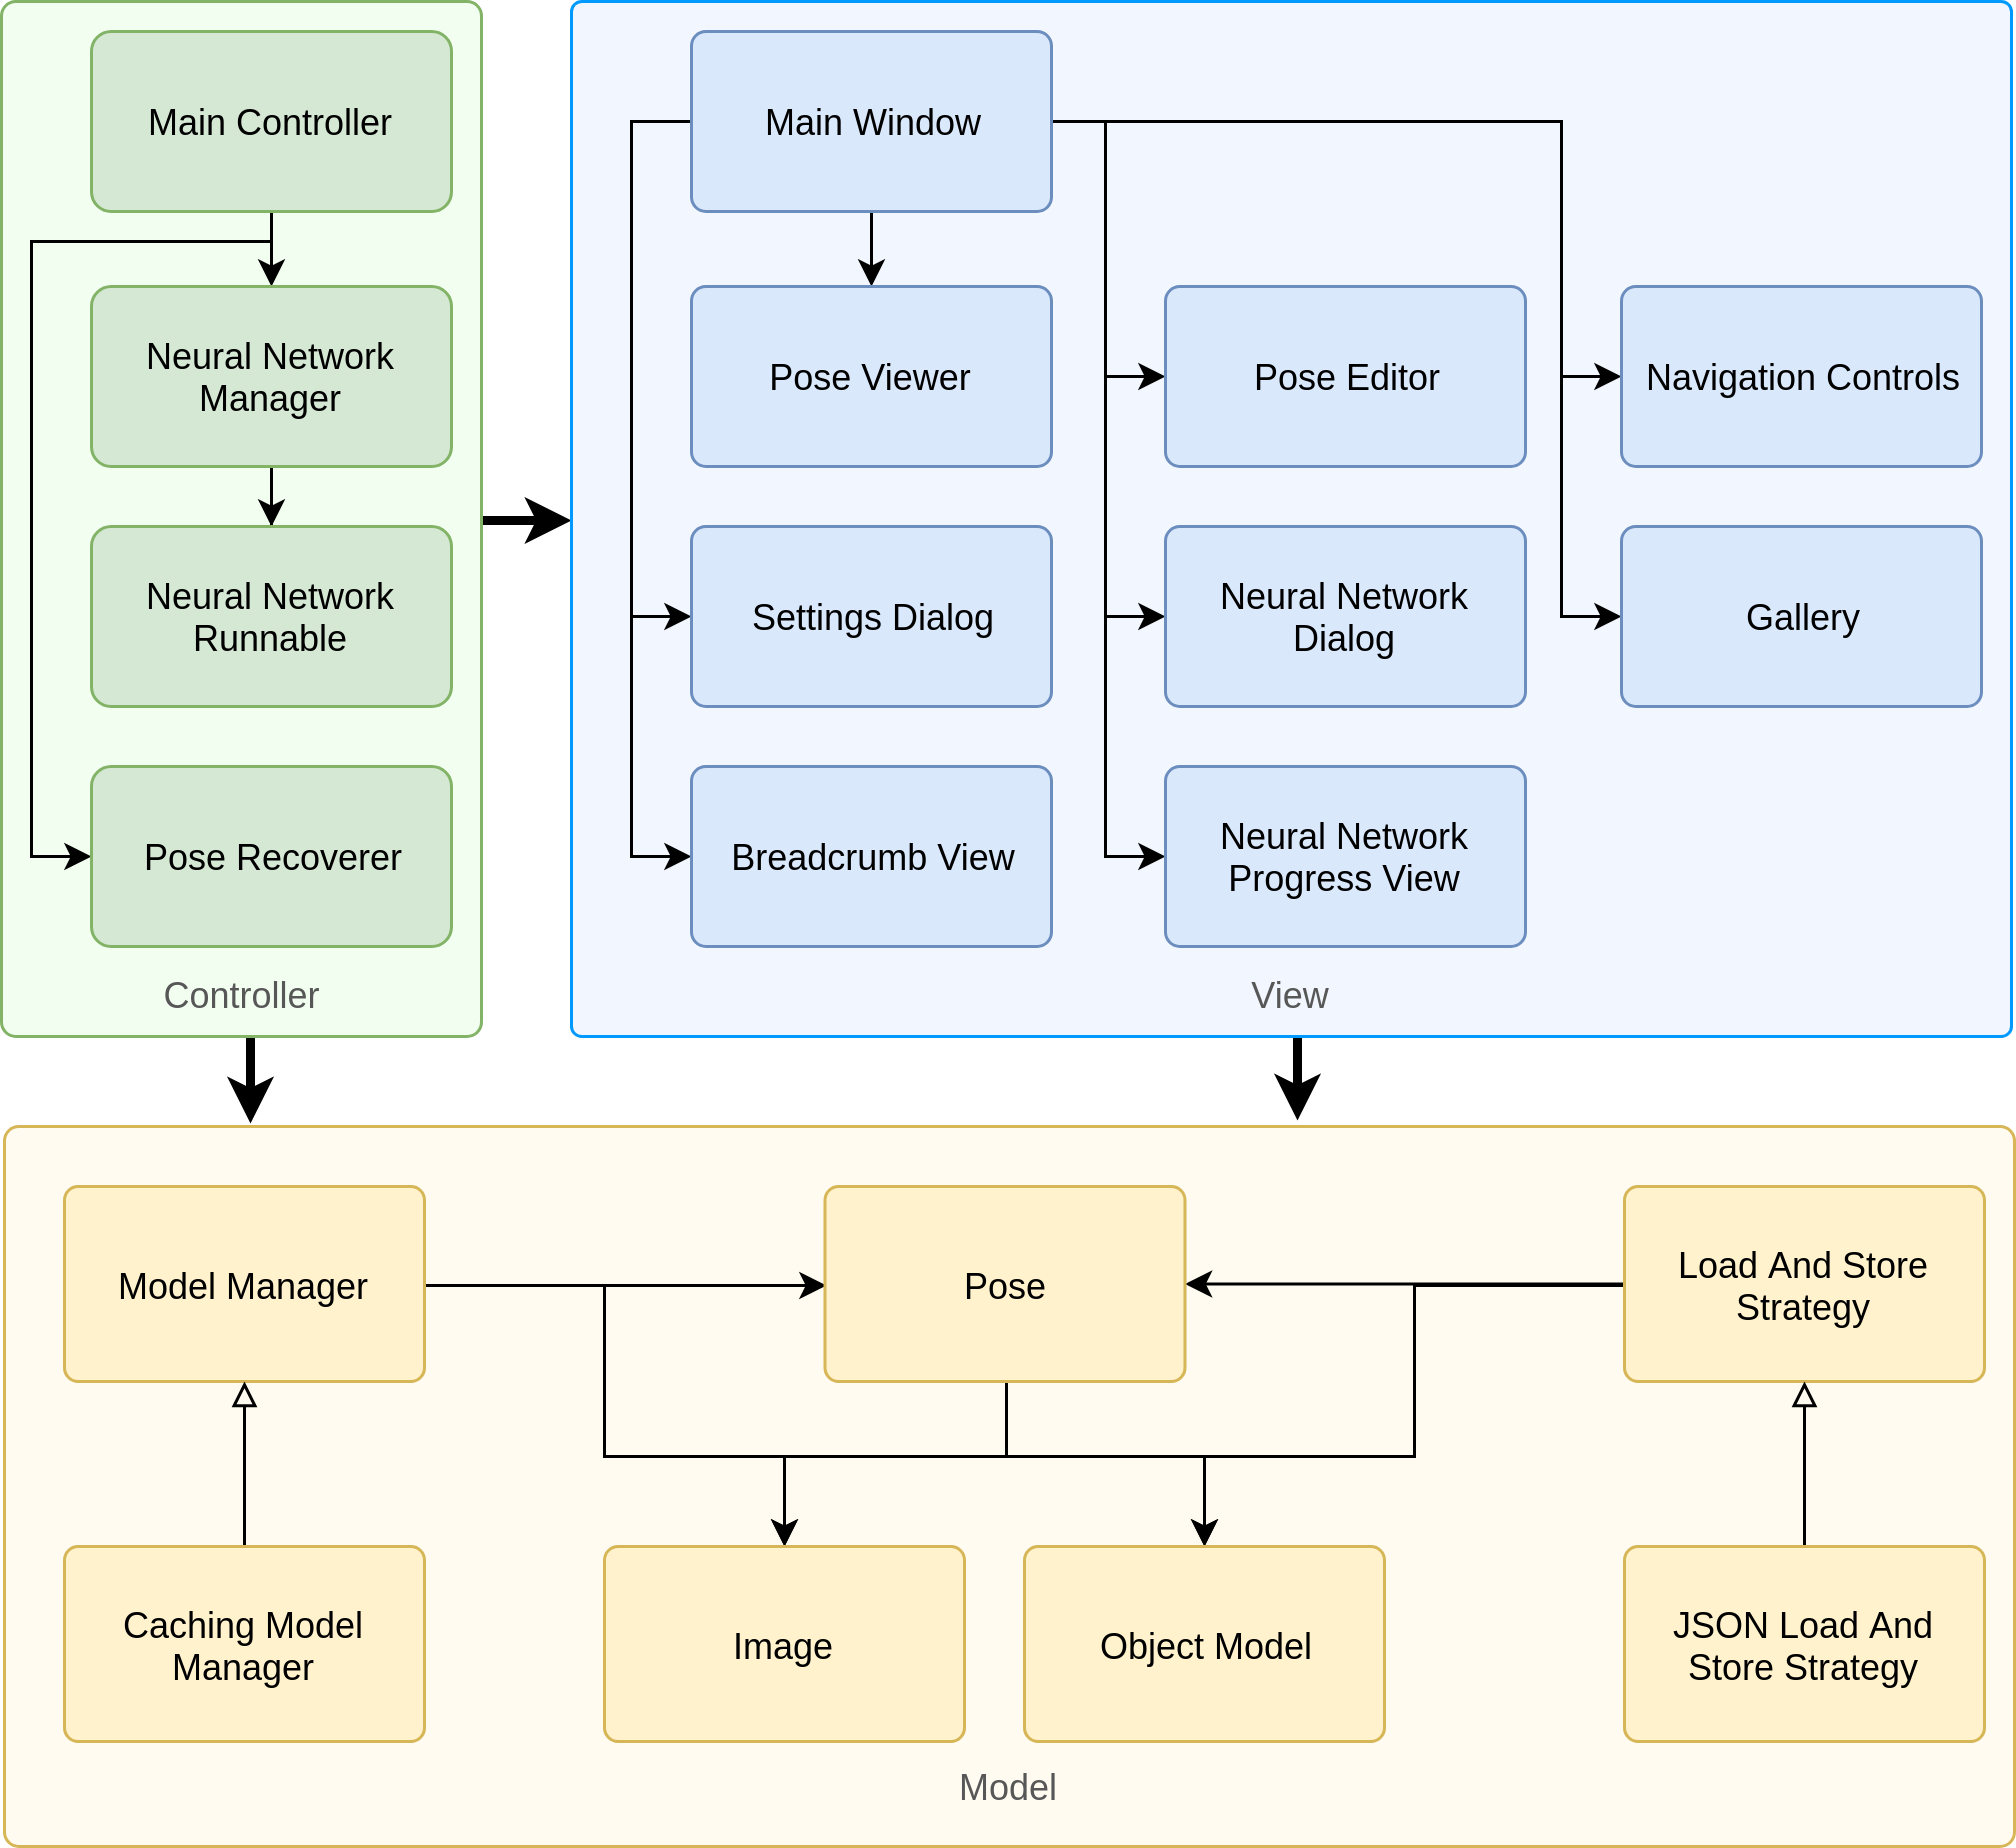
\includegraphics[width=0.9\linewidth]{6dpat_class_diagram}
    \caption{An abstract high-level class diagram of a subset of the classes of \gls{6dpat}. The \textbf{Main Controller} holds the references to the \textbf{Pose Recoverer}, the \textbf{Neural Network Manger} and the \textbf{Neural Network Runnable}. The Pose Recoverer stores the clicked 2D-3D correspondences and implements functionality to recover a pose. The Neural Network Manager controls the connection to the neural network and uses the Neural Network Runnable to execute network tasks. The Main Controller also owns the \textbf{Main Window}, which consists mainly of the classes visible in the "View" rectangle. The \textbf{Pose Viewer} can display images and their poses and the \textbf{Pose Editor} can be used to edit those poses. The \textbf{Settings Dialog} allows editing of several preferences. To let the network predict poses, the user can open the \textbf{Neural Network Dialog} and select images to run prediction on. This opens the \textbf{Neural Network Progress View} until inference has finished. The \textbf{Breadcrumb View} shows the currently set folders to load images and object models from. The \textbf{Navigation Controls} allow navigation through the \textbf{Galleries} showing the images and object models. The \textbf{Model Manager} uses the \textbf{Load And Store Strategy} to load images, object models and poses. The respective classes are depicted in the middle of the large rectangle labeled "Model". The Main Controller owns the Model Manager and passes it to the view classes. Own image.}
    \label{fig:6dpat_class_diagram}
\end{figure}

The most important C++ classes of the program are displayed in \fig \ref{fig:6dpat_class_diagram}. The diagram is simplified for easier understanding. The large rectangles group the classes by their affiliation in the MVC pattern. The bold arrows between the groups denote which classes can use or know which other classes. This does not necessarily mean, that all classes of the source rectangle use all classes of the target rectangle. The general structure of the program is the following: the main controller holds references to the \textit{Neural Network Manager}, the \textit{Pose Recoverer} and the \textit{Main Window}. The neural network manager uses the \textit{Neural Network Runnable} to execute training and inference tasks of the neural network. 

The pose recoverer manages the currently already clicked corresponding points and computes the new pose when requested and enough corresponding points are present. The main window consists of the two main widgets \textit{Pose Editor} and \textit{Pose Viewer}. The pose editor can display an object model $O$ selected from the objects \textit{Gallery} and allows editing all poses $P$ of an image $I$ selected from the images \textit{Gallery}. Both galleries are owned by the main window, as well. The pose viewer in turn renders all poses $P$ of an image $I$ onto the image. Pose viewer and editor can be used to recover poses by clicking corresponding points (see section \ref{subsection:correspondence_and_pose_creation}). 

The main window also uses the \textit{Breadcrumb Views} to display the paths that the user set to load images and object models from. The user can also navigate through the galleries via the \textit{Navigation Controls}. The \textit{Settings Dialog} can be opened to edit the preferences of the program. The user can open the \textit{Neural Network Dialog} and select the images to run the network prediction on. The main window then displays the \textit{Neural Network Progress View}. 

Most view classes use the model manager, the \textit{Image}, the \textit{Object Model} and the \textit{Pose} classes. The image class stores the paths to the actual image, as well as its segmentation counterpart. The path to the object model is maintained by the object model class. The pose class holds a reference to the respective image and object model and stores the rotation matrix and translation vector. 

The main controller sets the \textit{Load And Store Strategy} on the model manager. This class is responsible for reading imags and object models from the hard-drive, as well as persiting poses. The \textit{JSON Load And Store Strategy} uses the JSON format to store poses and read camera matrices. JSON is a format that is relatively easy for humans to read and is used by many deep learning applications. Transforming JSON formats can be done quickly and therefore provides the possibility to read data from other projects. The \textit{Caching Model Manager} is a simple implementation of the model manager interface that chaches images, object models and poses instead of delegating all loading calls to the strategy. 

The program offers functionality to start the network inference. We realized this feature by starting a new process. It is not necessary to use the official C++ Python bridge, since the network writes the predicted poses back to the target JSON file. This means that we do not need to retrieve any return values directly from the function call to the network inference.

\subsection{Manual Annotation} 

This sections describe the user interface of \gls{6dpat} and the required steps to annotate images with 6D poses. The user has to perform some steps before they can begin with the actual annotation process. 

\subsubsection{Preparation}

\begin{figure}[!tbp]
	\centering
	\begin{subfigure}[t]{\textwidth}
		\centering
    	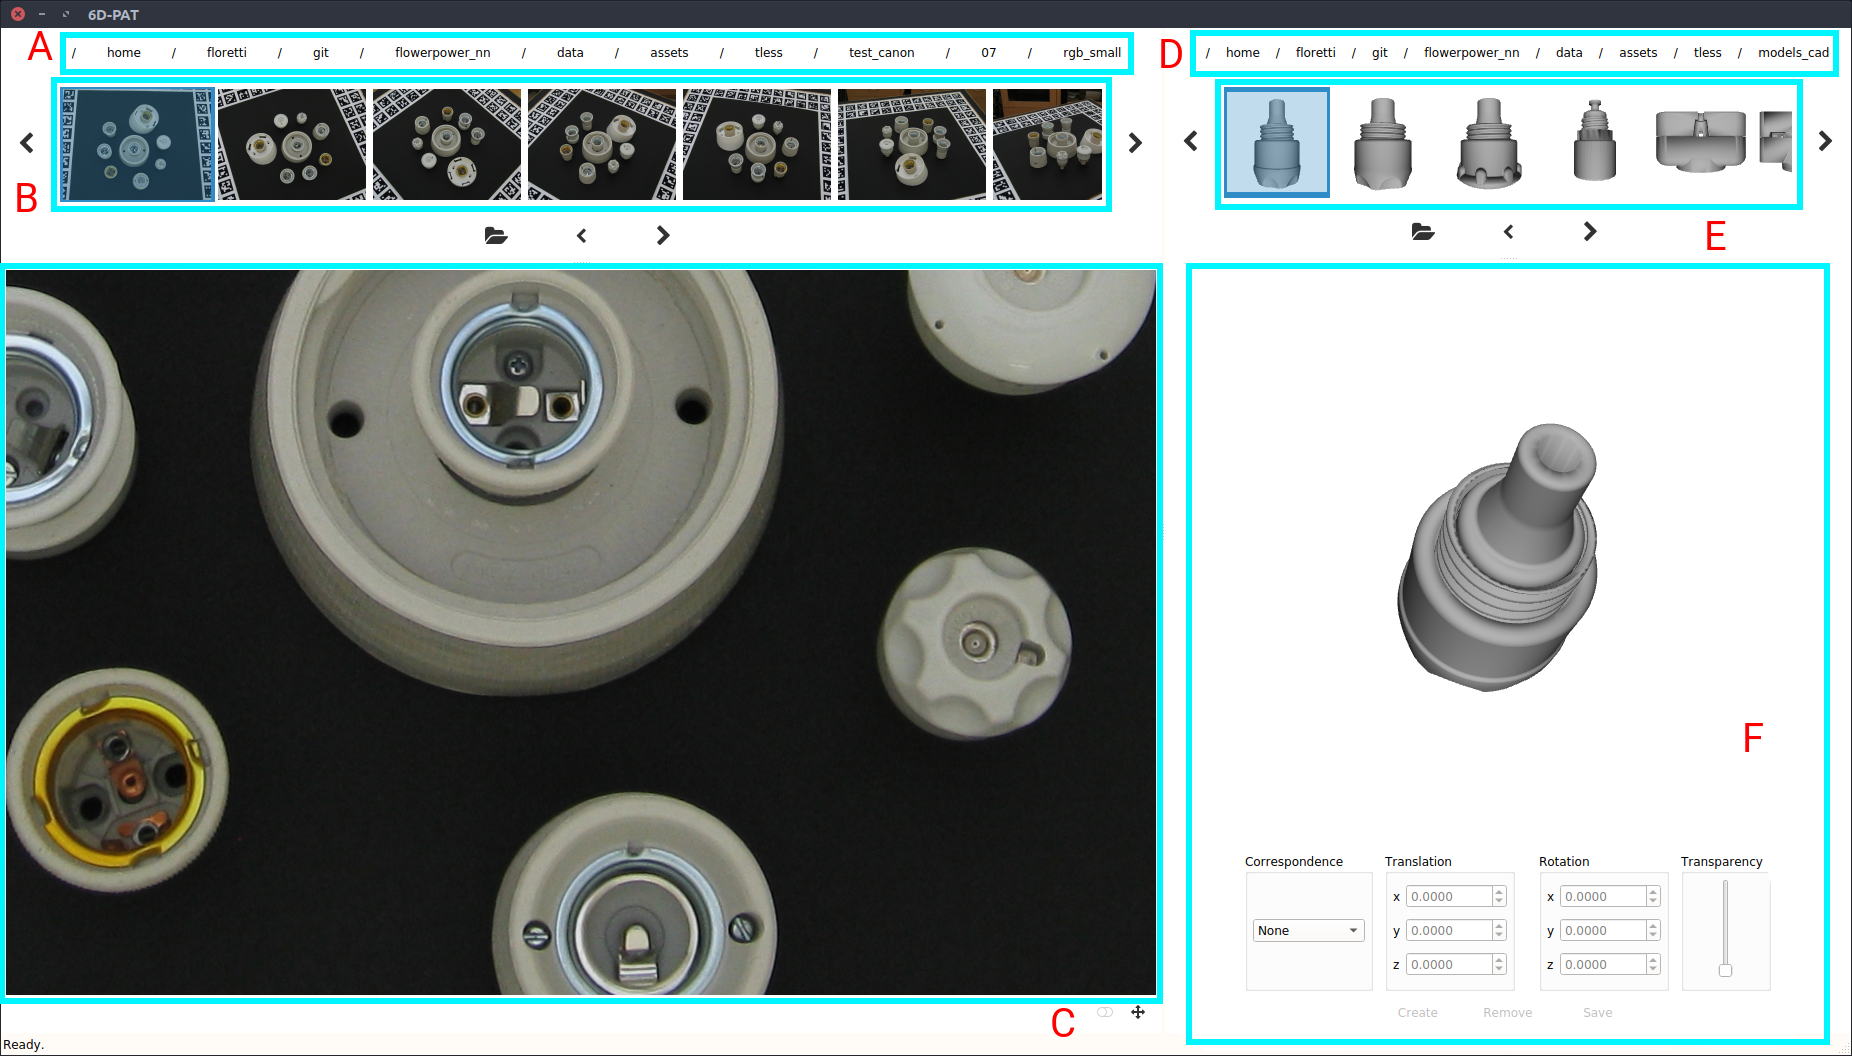
\includegraphics[width=\linewidth]{6dpat_components}
    	\caption{The user interface of the annotation tool \gls{6dpat}. The data displayed are images and object models from the T-Less dataset. The components marked with a turquoise box are the following ones: \textbf{A}: The full path of the currently selected folder to load images from. \textbf{B}: The gallery showing the images loaded from the selected path. \textbf{C}: The \textit{Pose Viewer} shows the image selected in gallery B. The user can click on the image to define the 2D starting point of a correspondence. \textbf{D}: The full path of the currently selected folder to load object models from. \textbf{E}: The gallery of rendered 3D preview of the object models loaded from the selected path. \textbf{F}: The \textit{Pose Editor} shows the object model selected in gallery E. The user can click on the object model to complete the correspondence with the 3D point. The controls at the bottom can be used to edit existing poses. Own image.}
    	\label{fig:6dpat_components}
	\end{subfigure}
	\par\bigskip
	\begin{subfigure}[t]{0.47\textwidth}
		\centering
    	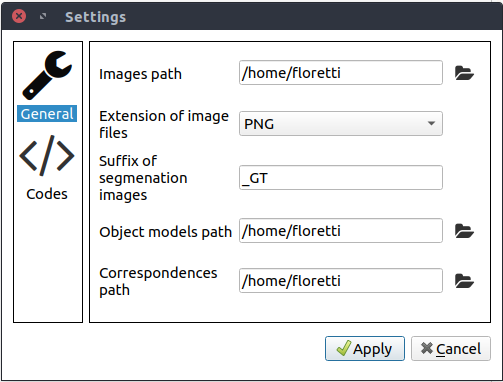
\includegraphics[width=0.8\linewidth]{6dpat_settings}
    	\caption{The settings dialog of \gls{6dpat}. The dialog allows editing of the paths where the program loads images, object models and poses from. Own image.}
    	\label{fig:6dpat_settings}
	\end{subfigure}
	\hfill
	\begin{subfigure}[t]{0.47\textwidth}
	\centering
    	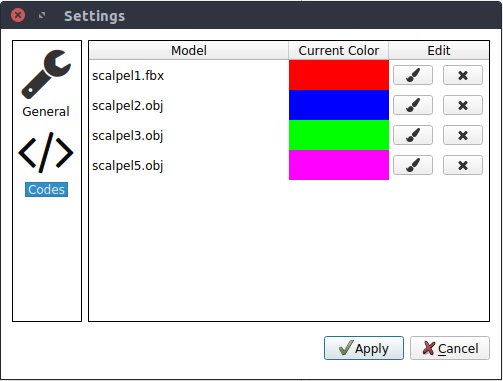
\includegraphics[width=0.8\linewidth]{6dpat_settings_codes}
    	\caption{The tab of the settings dialog that can be used to assign colors to the object models. Own image.}
    	\label{fig:6dpat_settings_codes}
	\end{subfigure}
	\caption{The main view of \gls{6dpat} as well as the two settings views.}
	\label{fig:6dpat_ui_overview}
\end{figure}

The first step after starting the program is to open the settings (see \fig \ref{fig:6dpat_settings}) and set the path to the images that are to be annotated, as well as the path to the folder that contains the object models that are visible in the images. 

The folder of the images has to contain a JSON file that holds the camera matrix $K$ for each individual image. If no camera info file exists, a Python script that is distributed with the neural network can be used to created approximate camera matrices. The path to the segmentation images (if any) has to be set as well. The program loads the images and the segmentation images and sorts them by the numbers in their filenames and then matches image $I$ at index $j$ with the segmentation image $S$ at index $j$. 

Lastly, the user needs to specify the location of the JSON file where the program is supposed to load existing ground-truth poses from and write new ones to. If no such file exists an empty one can be created and selected. If segmentation images are present they are linked to the respective image and can be viewed by activating the toggle at the bottom right corner of the pose viewer (the program displaying a segmentation image can be seen in \fig \ref{fig:sfb_segmentation}). 

If required, the user can assign colors to the object models using the tab of the settings dialog depicted in \fig \ref{fig:6dpat_settings_codes}. The colors should correspond to the respective color used in the segmentation mask. The object models gallery will automatically display only the object models whose color is present in the segmentation image of the currently viewed image. If no segmentation images exist, then the gallery shows all object models.

\subsubsection{Correspondences Creation and Pose Recovery} \label{subsection:correspondence_and_pose_creation}

\begin{table}
\centering
    \begin{tabular}{|c||ccccc|} \hline
\diagbox{\# Object}{Image} & 0000.jpg & 0150.jpg & 0250.jpg & 0350.jpg & 0500.jpg \\ \hline\hline
01           &  2:30 min & 1:23 min & 2:05 min & 3:06 min & 0:50 min \\ 
        15 & 2:16 min & 1:51 min & 1:35 min & 2:20 min & 3:07 min \\ \hline
\end{tabular}
	\caption{Example times for annotating images with poses of objects. The images were taken from the test scene 7 of the T-Less dataset. The provided times are the measurements for recovering a single pose of the respective object. The numbers are supposed to give an impression of the efficiency of the program. Poses were accepted as correct when they were deemed close enough to the existing ground-truth pose. Own table.} 
	\label{tabel:6dpat_example_times}
\end{table}

The component corresponding to the letters that we use in the following paragraph can be taken from \fig \ref{fig:6dpat_components}. To annotate a new pose, the user has to select an image $I$ from gallery \textit{B}, first. The pose viewer \textit{C} then displays the image. The model $O$ that the image is to be annotated with can be selected from the gallery \textit{E}. The pose editor \textit{F} shows the selected object model. The user can rotate the object to view otherwise hidden areas. The arrow keys can be used to move the object along the $x$ and $y$ and also, if the shift key is pressed, along the $z$ axis. 

When the object is in an appropriate position, the user can begin to create a correspondence $C$ by clicking on $I$. This defines the 2D location $u$ of the correspondence. To complete the correspondence, the object model $O$ has to be clicked at the respective position $p$. This procedure has to be repeated until enough correspondences have been defined to create the new pose $P$. The minimum is 4 correspondences. 

The creation process is shown in \fig \ref{fig:6dpat_correspondence_creation}. More correspondences can make the initial pose more accurate. Clicking the "Create" button at the bottom of the pose viewer creates the pose $P$ using the correspondences $C_i$ and OpenCV's \textit{solvePnPRansac} method. The newly created pose can be refined using the controls of the pose viewer. After pose refinement it is necessary to click the "Save" button. 

The slider labeled "Transparency" can be used to reduce the object's opacity on the image. After all poses have been annotated successfully the next image can be selected from the gallery B. This operation has to be repeated until the dataset is fully annotated, although intermediate states can be used to train the network already (see chapter \ref{chapter:semi_automatic}).

It is possible to use the neural network to predict poses. This requires a proper setup and training of the network beforehand. The user can then start the prediction process by clicking the "Predict" button in the lower right corner of the pose editor.

Example times of the manual (without the network) annotation process are given in Table \ref{tabel:6dpat_example_times}. The images were taken from the T-Less dataset, test scene 7. The times state how long it took the author to recover a single pose for an object. The numbers are just supposed to give an impression. Poses were deemed correct when within an subjectively acceptable range of the existing ground-truth pose provided by T-Less.

\begin{figure}[!tbp]
	\centering
    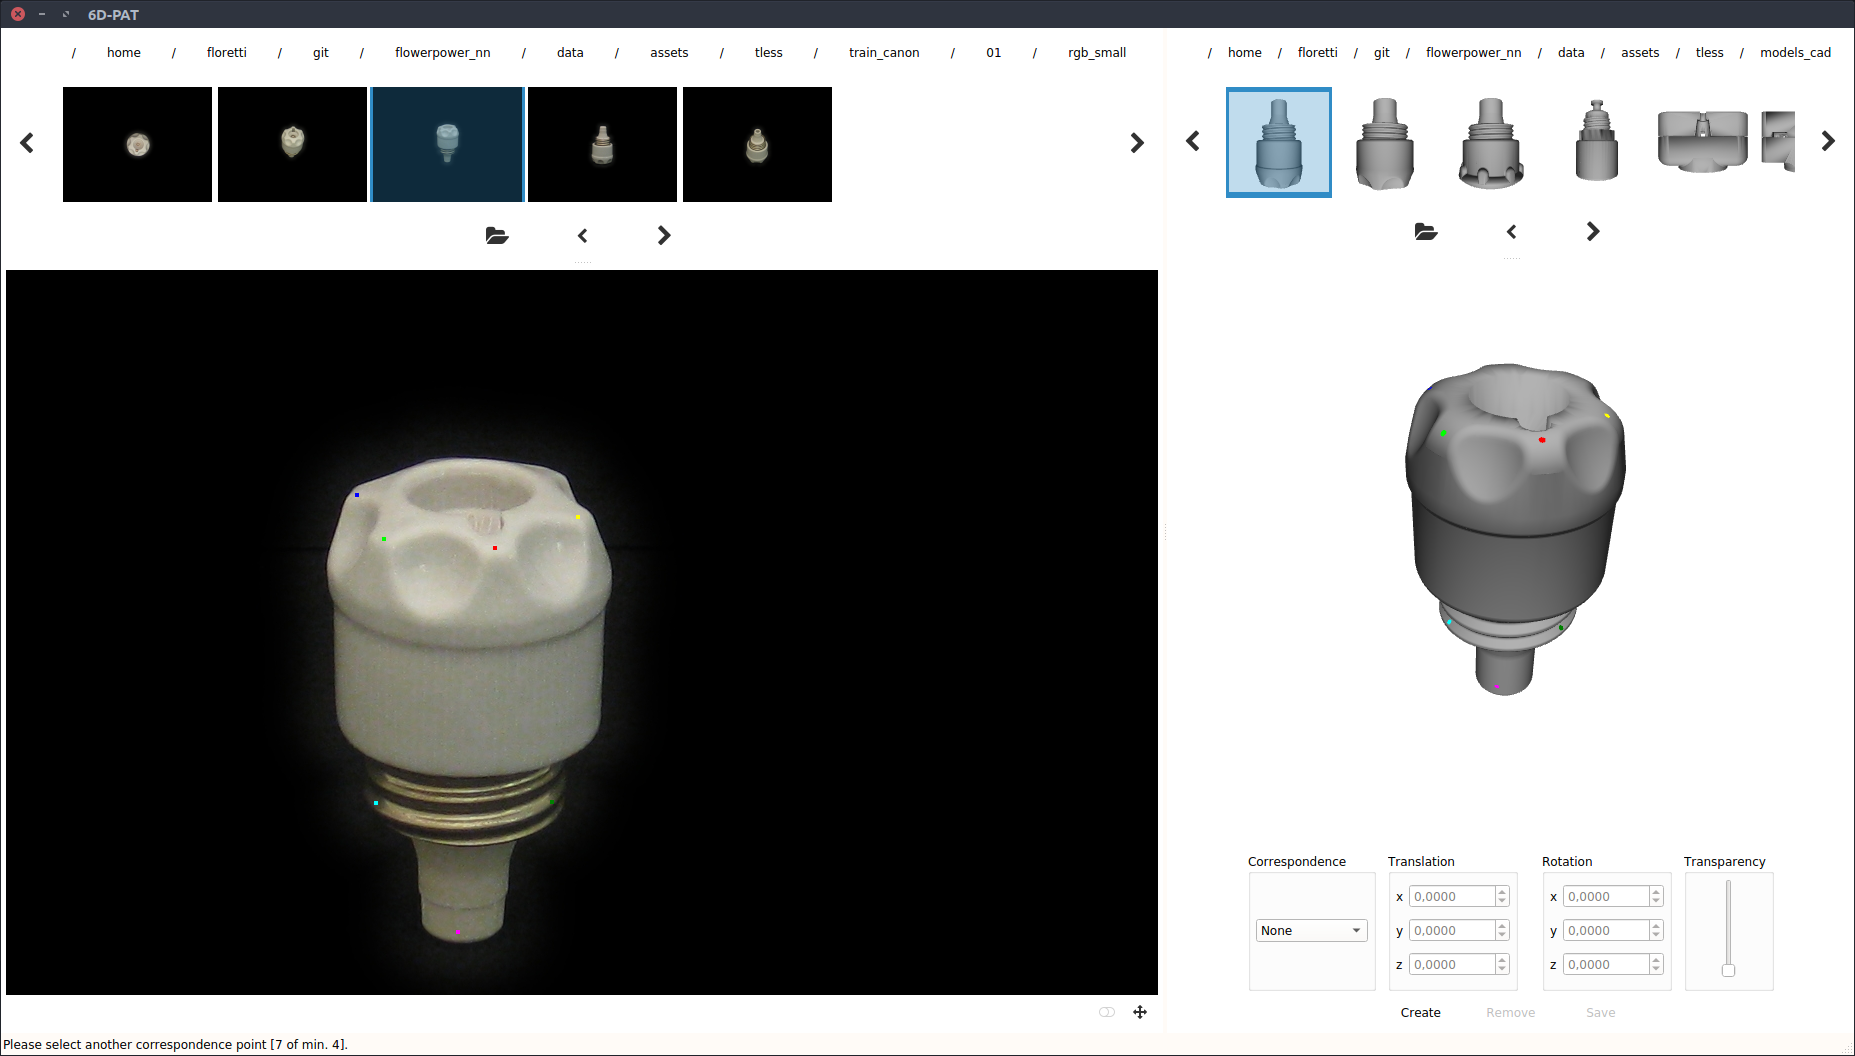
\includegraphics[width=\linewidth]{6dpat_correspondence_creation}
    \caption{The pose creation process. The user has to click the image first and then the corresponding 3D location on the object model. The red circles and red lines were added afterwards to emphasize the colored dots which the program draws. Own image.}
    \label{fig:6dpat_correspondence_creation}
\end{figure} 

\subsection{Problems \& Difficulties} \label{section:6dpat_difficulties}

During the implementation of the program multiple problems arose and complicated the development process. We summarize the most important ones and explain issues which contradicted the intended usage patterns and impacted the final design.

One of the major factors that prolong the implementation process was that we tried to realize all graphical processing using the \textit{Qt3D} framework, which is part of the main Qt framework. Qt3D's purpose is to encapsulate graphics programming to increase portability of applications including 3D graphics. The incomplete documentation and unintuitive concepts make it difficult to use without consultation. After complications still emerged in the almost completed annotation tool the Qt3D framework was deemed unusable and omitted in favor of a native OpenGL implementation.

Initially, a desired feature of the program was to present a next unannotated image when the user annotated all poses of an image. This is not feasible for multiple reasons. First of all, a user might still not be content with the poses. Selecting the next image programmatically could happen to early and disrupt the annotation process of the user.

The datasets to annotate can also have very distinct characteristics, which require the user to choose the next image personally. For a dataset like T-Less, many images have to be skipped due to their similarity. Intuitively, the more diverse poses are annotated, the better a neural network can be trained. Instead of forcing the user to annotate varying images the motivation should be the faster annotation process as soon as the neural network is able to make plausible predictions. 

The diversity of available dataset (see Chapter \ref{chapter:experiments}) is also the reason why the program does not provide functionality to initialize the next poses based on the ones in the last image. This feature would imply too many assumptions on the dataset and, in the worst case, cause more work for the user. 

While trying to annotate the images of the Endoscopic Vision Challenge dataset it became clear, that proper 3D models are crucial for successful annotation. To temporarily annotate the medical images, 3D surgical tools were downloaded from the internet as a replacement for the missing object models. But having a different shape and also missing the distinctive features of the real objects makes it very difficult to estimate the ground-truth pose. The influence of contradicting annotated poses during training of a network is not clear. The author of this work strongly recommends to obtain the correct 3D models before annotating the Endoscopic Vision Challenge images. The issue of the object models not fitting the segmentation mask can be seen in \fig \ref{fig:sfb_segmentation}. \fig \ref{fig:sfb_original} shows the actual image and the discrepancy between the object models and image pixels.

\begin{figure}[!tbp]
	\begin{subfigure}[t]{0.47\textwidth}
		\centering
    	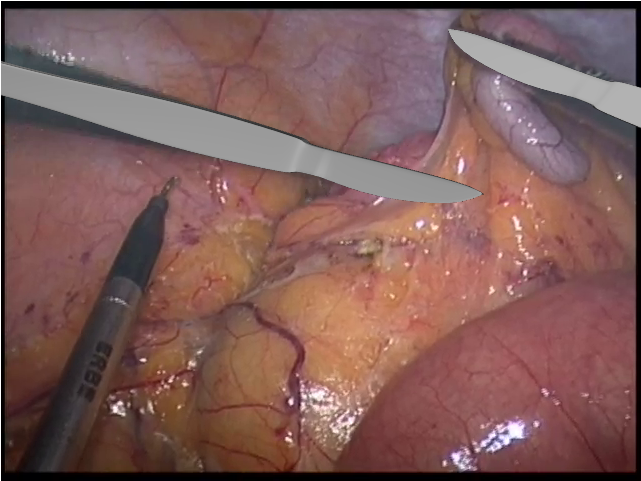
\includegraphics[width=\linewidth]{6dpat_sfb_image}
    	\caption{An image from the medical images dataset annotated using 6D-PAT. The correct rotation and translation are difficult to estimate without the actually used tools. Own image.}
    	\label{fig:6dpat_sfb_image}
	\end{subfigure} 
	\hfill
	\begin{subfigure}[t]{0.47\textwidth}
		\centering
    	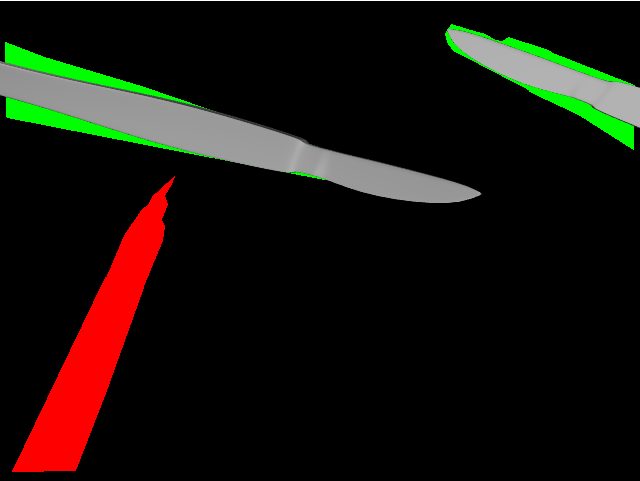
\includegraphics[width=\linewidth]{6dpat_sfb_segmentation}
    	\caption{The corresponding segmentation image to the image on the right. The discrepancy between the segmentation masks and the object model is clearly visible as the green area. Own image.}
    	\label{fig:6dpat_sfb_segmentation}
	\end{subfigure} 
\end{figure} 

A first try to use the official Python bindings did not work to our complete satisfaction. The rather involved alterations to the program to be able to handle the Python script running inference are too complex compared to starting an external process. Qt offers this functionality to start a process, already.

The Python binding is not complete yet. Training is not possible and the a deep learning expert has to setup the network and its parameters to enable its usage in the program. The current state of the incorporation of the network is to be seen as a proof of concept that requires further development.

Because the neural network is trained only for one object, the time-intensive step (proportional to the overall time needed for inference on one image) of loading the trained weights has to be performed each time when running inference for different objects. The frame of this work was to explore neural networks trained for one object only, it is therefore not known whether this overhead of loading the weights can be reduced.

\subsection{Future Improvements of \gls{6dpat}}

To provide an outlook how the program can be improved in the future, we mention solutions to some of the problems of Section \ref{section:6dpat_difficulties}. An important feature that should be implemented is moving the object models around on the displayed image by dragging and rotating them with the mouse. The initial poses of the models using the clicking procedure are pretty accurate in many cases already. But sometimes, when the camera is looking along an axis of the object, the rotation is far off. The user can correct the poses with the provided controls. But using them takes some skill and time. The described editing process would profit in terms of time needed per annotation. To give the user a better overview over the image and its annotated poses, a zoom option should be implemented, as well.

The binding of the neural network to the program does not allow to load the weights of the net and persist this state in the memory of the computer. In case that the user wants to annotate a large dataset of just one object, they could profit from a feature allowing to keep the weights in memory instead of loading them each time the inference process is started. This way, predicting the pose for only one image could be achieved in significantly less time.

Another suggested step is to fully incorporate the network in the annotation tool. This way inexperienced users can profit from the network without the need for an expert every time they want it to detect poses in an image. There is probably no way to automatize setting up the network as this requires knowledge of neural nets. In an ideal setting it can be kept to a minimum and users can be introduced to the most relevant parameters, which they can set from within the program.